\adparagraph{Kendall Tau Distance}
Looking at Figure \ref{fig:kendalldistance} we can see the results of the Footrule distance test. As mentioned in Section \ref{sec:distance} \note{remember to mention is in the section} the distanced measures have a score between 0 and 1 where 0 correspond to equal lists and 1 denotes that the lists are reverse of each other or containing different items.\note{This is not all true since a list with all different items scores 0.7778} 

A general trend when looking at the graph is that all the methods follow the same curve where there is a somewhat large difference of around 0.06 between group sizes 4 and 8. However as the groups grow the increase in the Kendall distance fades out and becomes very low and the difference between 20 and 40 is approximately 0.006. 

Looking at the approaches individually Average clearly scores the highest. The reason is that Average disregards the item ranks in the top-k lists and aggregates them based on the average rating between the group members instead.  
   
Next we have SF. This is surprising because, within the information retrieval domain, SF usually perform notably better than BC does. \note{Find cite for this} We do not have a reasonable explanation for why this is the case, but we expect it to have something to do with \note{Why??}

Lastly performing best and somewhat equal we have BC and MC. Worth noting is that when the groups are small MC performers slightly best, but as the groups grow the differers between the performance decreases and BC ends op out scaling MC when the group size is around 12.

%The reason the scores in this case are lower then those for Footrule is that its an average scor meaing that it is potential better to not have an item on the list than in revers order. 

\begin{figure}[H]
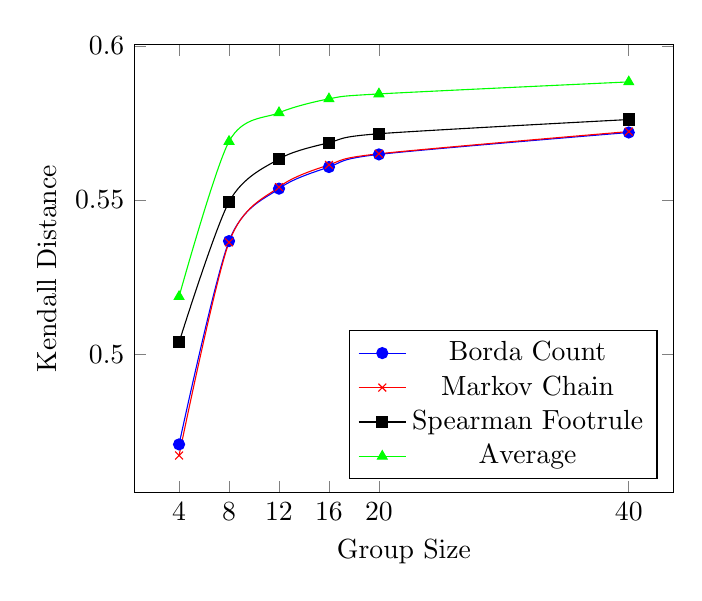
\begin{tikzpicture}
    \begin{axis}[
        xlabel=Group Size,
        ylabel=Kendall Distance,
        xtick = {4,8,12,16,20,40},
        legend pos=south east]
    \addplot[smooth,mark=*,blue] plot coordinates {
        (4,0.4708)
        (8,0.5367)
        (12,0.5537)
        (16,0.5607)
        (20,0.5648)
        (40,0.5719)
    };
    \addlegendentry{Borda Count}

    \addplot[smooth,color=red,mark=x] plot coordinates {
            (4,0.4672)
            (8,0.5363)
            (12,0.5542)
            (16,0.5614)
            (20,0.565)
            (40,0.5722)
        };
    \addlegendentry{Markov Chain}
    
        \addplot[smooth,color=black,mark=square*] plot coordinates {
            (4,0.5039)
            (8,0.5494)
            (12,0.5633)
            (16,0.5686)
            (20,0.5715)
            (40,0.5761)
        };
    \addlegendentry{Spearman Footrule}
    
    \addplot[smooth,color=green,mark=triangle*] plot coordinates {
            (4,0.5187)
            (8,0.569)
            (12,0.5783)
            (16,0.5828)
            (20,0.5844)
            (40,0.5883)
        };
    \addlegendentry{Average}
    
    \end{axis}
\end{tikzpicture}
\caption{Results using Kendall Tau distance} \label{fig:kendalldistance}
\end{figure}